\documentclass[a4paper,12pt,oneside]{article}
\usepackage{amsmath}
%\usepackage{mathtools}
\usepackage{caption}
\usepackage{mathptmx}
\usepackage{fixltx2e}
\usepackage{graphicx}
\usepackage[margin=1.0in]{geometry}
\usepackage{float}
\usepackage{setspace}
\usepackage{chngcntr}
\usepackage{fancyhdr}
\pagestyle{fancy}
\fancyhf{}
\rfoot{\thepage}
%\renewcommand{\headrulewidth}{0.0pt}
%\renewcommand{\footrulewidth}{0.0pt}

\begin{document}
\thispagestyle{empty}
%\pagenumbering{gobble}
\begin{center}

\large{\textbf{{FINGERPRINT LIVENESS DETECTION USING CONVOLUTIONAL NEURAL NETWORK}}}
\setlength{\baselineskip}{1.5\baselineskip}
\\

\vspace{5mm}
\textbf{SEMINAR REPORT}

Submitted in the partial fulfilment of the award of the degree
of
\\
\textbf{Bachelor of Technology}
\\
in
\\
\textbf{Computer Science \& Engineering}
\\
of
\\
\textbf{APJ Abdul Kalam Technological University}
\\
by
\\
\textbf{JICKCY ANNA KOSHY}
\\
\vspace{5mm}
\begin{figure}[H]
	\centering
	
\includegraphics{ceclogo.png}
\end{figure}
\textbf{November, 2018}
\vspace{8mm}
\\
Department of Computer Engineering
\\
College of Engineering, Chengannur, Kerala -689121
\\
Phone: (0479) 2454125, 2451424; Fax: (0479) 2451424
\\



\end{center}
\newpage
\thispagestyle{empty}
\begin{center}
\setlength{\baselineskip}{1.5\baselineskip}
{\large\textbf{COLLEGE OF ENGINEERING, CHENGANNUR}}
\\
{\large\textbf{KERALA}}
\\
\begin{figure}[H]
\centering

\includegraphics{ceclogo.png}
\end{figure}
\setlength{\baselineskip}{1.5\baselineskip}
\textbf{Department of Computer Engineering}
\\
\textbf{CERTIFICATE}
\\
This is to certify that the seminar entitled
\\
\textbf{FINGERPRINT LIVENESS DETECTION USING CONVOLUTIONAL NEURAL NETWORK}
\\
Submitted by
\\
\textbf{JICKCY ANNA KOSHY}
\\
is a bonafide record of the work done by her.
\end{center}
\vspace{14ex}
%\textbf{Mrs.Sheeba}
\hspace{55ex}
%\textbf{Dr. Smitha Dharan}
\\
\vspace{2ex}
\hspace{0ex}
\textbf{
Co-ordinator}
\hspace{45ex}
\textbf{
Head of The Department}
\newpage
\pagenumbering{roman}


\renewcommand{\headrulewidth}{0.0pt}
\renewcommand{\footrulewidth}{0.0pt}



\begin{center}
\large{\textbf{ACKNOWLEDGEMENT}}
\end{center}
\vspace{6ex}
\setlength{\baselineskip}{1.5\baselineskip}

\paragraph{}
I am greatly indebted to God Almighty for being the guiding light throughout with his
abundant grace and blessings that strengthened me to do this endeavour with confidence.
\paragraph{}
I express my heartfelt gratitude towards \textbf{Dr. Jacob Thomas V.}, Principal, College
of Engineering Chengannur for extending all the facilities required for doing my seminar.
I would also like to thank \textbf{Dr. Smitha Dharan}, Head, Department of Computer
Engineering, for providing constant support and encouragement.
\paragraph{}
Now I extend my sincere thanks to my seminar co-ordinators \textbf{Mr. Gopakumar G.}, Associate
Professor in Computer Engineering and \textbf{Ms. Meera Varma} , Assistant
Professor in Computer Engineering for guiding me in my work and providing timely
advices and valuable suggestions.
\paragraph{}
Last but not the least, I extend my heartfelt gratitude to my parents and friends for
their support and assistance.	

\pagenumbering{gobble}
\newpage

\begin{center}
\large{\textbf{ABSTRACT}}
\end{center}
\vspace{6ex}
\paragraph{}

With the growing use of biometric authentication
systems in the recent years, spoof fingerprint detection has become increasingly important. In this study, we use Convolutional Neural Networks (CNN) for fingerprint liveness detection. Our system is evaluated on the datasets used in The Liveness Detection Competition of years 2009, 2011 and 2013, which comprise almost 50,000 real and fake fingerprints images.  Dataset Augmentation is used to increase the classifiers performance, not only for deep architectures but also for shallow ones. We also report good accuracy on very small training sets (400 samples) using these large pre-trained networks. Our best model achieves an overall rate of 97.1\% of correctly classified samples - a relative improvement of 16\% in test error when compared with the best previously published results

\setlength{\baselineskip}{1.0\baselineskip}
\newpage
\begin{center}
\tableofcontents
\end{center}
\newpage
\thispagestyle{plain}
\begin{center}
\listoffigures
\end{center}





\newpage
\rfoot{\thepage}

\lhead{\textit{Fingerprint Liveness Detection Using 
Convolutional Neural Network}}

\lfoot{\textit{College of Engineering, Chengannur}}

\rfoot{\thepage}

\renewcommand{\headrulewidth}{0.0pt}
\renewcommand{\footrulewidth}{0.0pt}




\renewcommand{\headrulewidth}{0.0pt}
\renewcommand{\footrulewidth}{0.0pt}



\section{INTRODUCTION}
\pagenumbering{arabic}
\paragraph{}
The basic aim of biometrics is to automatically discriminate subjects in a reliable manner for a target application based on one or more signals derived from physical or behavioral traits, such as fingerprint, face, iris, voice, palm, or handwritten signature. Biometric technology presents several advantages over classical security methods based on either some information(PIN, Password, etc.) or physical devices (key, card, etc.) [2]. However, providing to the sensor a fake physical biometric can be an easy way to overtake the systems security. Fingerprints, in particular, can be easily spoofed from common materials, such as gelatin, silicone, and wood glue [2]. Therefore, a safe fingerprint system must correctly distinguish a spoof from an authentic finger (Figure 1). Different fingerprint liveness detection algorithms have been proposed [3], [4], [5], and they can be broadly divided into two approaches: hardware and software. In the hardware approach, a specific device is added to the sensor in order to detect particular properties of a living trait such as blood pressure [6], skin distortion [7], or odor [8]. In the software approach, which is used in this study, fake traits are detected once the sample has been acquired with a standard sensor.
\paragraph{}
The features used to distinguish between real and fake
fingers are extracted from the image of the fingerprint. There
are techniques such as those in [2] and [9], in which the
features used in the classifier are based on specific fingerprint
measurements, such as ridge strength, continuity, and clarity.Convolutional Neural Networks were used to detect false vs real fingerprints. Pre-trained CNNs can yield state-of-the-art results on benchmark datasets without requiring architecture or hyper parameter selection. We also showed that these models have good accuracy on very small training sets (˜400 samples). Additionally, no task-specific hand-engineered technique was used as in classical computer vision approaches. Despite the differences between images acquired from different sensors, we show that training a single classifier using all datasets helps to improve accuracy and robustness. This suggests that the effort required to design a liveness detection system (such as hyper-parameters fine tuning) can be significantly reduced if different datasets (and acquiring devices) are combined during the training of a single classifier. Additionally, the pre-trained networks showed stronger generalization capabilities in cross-dataset experiments than CNN with random weights and the classic LBP pipeline.




\newpage
\section{LITERATURE REVIEW}
\paragraph{}
\textbf{Fingerprint Recognition Using Genetic Algorithm and Neural Network} \textit{Purneet Kaur , Jaspreet Kaur}[10] In this paper,feature selection method is based on Genetic algorithm. The fingerprint image is enhanced before extracting features. Enhancement method included histogram equilization, binarization, morphological operations, it has made a great improvement of recognition accuracy for recognition method. The combination of both genetic algorithm and neural network techniques provided the better and efficient method for fingerprint biometric. Experimental results show that the presented method has the better recognition accuracy compared with the previous fuzzy logic based recognition methods.
 
\paragraph{}
\textbf{Fingerprint Recognition and Matching }\textit{Aliyu Tukur
}[11] The reliability of any automatic fingerprint verification system strongly relies on the precision obtained in the minutia extraction process. A number of factors damage the correct location of minutia. Among them, poor image quality is the one with most influence. The proposed minutiae matching algorithm is  capable of finding the correspondences between minutiae without resorting to exhaustive research. However, there is a scope of further improvement in terms of efficiency and accuracy which can be achieved by improving  the hardware to
capture the image or by improving the image enhancement techniques.






\paragraph{}
\textbf{Fingerprint identification and recognition using backpropagation neural network}\textit{ Adrian Lim Hooi Jinl, Ai Chekima, Jamal Ahmad Dargham, and Liau Chung Fan}[12] In this paper, to enhance the system constructed features
extraction has to be implemented inside this system.
Here features extracted from the
fingerprint image can be classified into local features
and global features, thus increasing the accuracy of
further fingerprint identification and recognition
process. After the image has been processed it
would then be fed into the back propagation neural
network as input in order to train the network. After
training, the neural network is ready to perform the
identification and recognition operations (matching
process). A neural network has been necessarily
developed to identify and recognize the core part of
the fingerprint images.
\paragraph{}
\textbf{Fingerprint Spoof Detection Using Contrast
Enhancement and Convolutional
Neural Networks}\textit{Han-Ul Jang, Hak-Yeol Choi, Dongkyu Kim, Jeongho Son,and Heung-Kyu Lee }[13] In this paper, we propose a technique to detect fingerprint spoof using contrast enhancement and CNN.Here uses histogram equalization as a contrast enhancement technique to improve the recognition rate of fingerprint images and detects fake fingerprints by judging whether or not the sub-block of fingerprint image is forged through CNNs. The proposed CNNs is composed of 6 weight layers and totalizing the results. The experimental results show that the average accuracy is 99.8%. Also, the detection method with contrast enhancement has relatively high performance improvement from 98.83% to 99.8%.


\paragraph{}
\textbf{Fingerprint Liveness Detection
based on Weber Local Image Descriptor}\textit{Diego Gragnaniello, Giovanni Poggi, Carlo Sansone and Luisa Verdoliva} [14]In this paper, we investigate the use of a local discriminative feature space for fingerprint liveness detection. In particular, we rely on the Weber Local Descriptor (WLD),
which is a powerful and robust descriptor recently proposed for texture classification. Inspired by Weber’s law, it consists of two components, differential excitation and orientation, evaluated for each pixel of the image. Joint histograms of these components are then processed to build the discriminative features used to train a linear kernel SVM classifier. Experimental results with different databases and different sensors show WLD to perform favorably compared to the state-of-the-art methods in fingerprint liveness detection. In addition, by combining WLD with LPQ (Local Phase
Quantization) results further improve significantly.

\paragraph{}
\textbf{Fingerprint Spoof Buster}\textit{Tarang Chugh, Kai Cao, and Anil K. Jain,}[15] A robust and accurate method for fingerprint spoof detection
is critical to ensure the reliability and security of the fingerprint
authentication systems. Here utilized
fingerprint domain knowledge by extracting local patches
centered and aligned using minutiae in the input fingerprint
image for training MobileNet-v1 CNN models. The local patch
based approach provides salient cues to differentiate spoof
fingerprints from live fingerprints. The proposed approach is
able to achieve a significant reduction in the error rates for
intra-sensor (63%), cross-material (43%), cross-sensor (4%)
as well as cross-dataset scenarios (29%) compared to state-ofthe-art
on public domain LivDet datasets.




\paragraph{}
\textbf{A Study of Biometric Approach Using Fingerprint
Recognition} \textit{ Ravi Subban and Dattatreya P. Mankame}[16] This paper presented the related works and performance
analysis for fingerprint biometric. The performance
evaluation is done on surveyed works with different
parameters and existing methods. Biometrics presents
obvious advantages over password and token-based security.
The survey study various issues related to uni-modal
biometric systems is discussed. The security and privacy
concerns that biometric authentication raises need to be
addressed. It is surveyed that automatic fingerprint
recognition is the best candidate biometric technology for
explosives security from an analysis of the requirements:
security, usability, ruggedness, size, form factor, privacy and
operational temperature range. 

\paragraph{}
\textbf{Fingerprint recognition using neural network}\textit{W. F. Leung, S. H. Leung, W. H. Lau and Andrew Luk }[17]This paper describes a neural network based approach for automated
fingerprint recognition. Minutiae are extracted from the fingerprint image via a multilayer perceptron (MLP) classifier with one hidden layer. The backpropagation learning technique is used for its training. Selected features are represented in a special way such that they are simultaneously invariant under shift, rotation and scaling. Simulation results are obtained with good detection ratio and low failure rate. The proposed method is found to be reliable for system with a small set of fingerprint data. 



\paragraph{}
\textbf{ Fingerprint Detection and Authentication using feature extraction based on Minutiae }\textit{
Hriday Goyal, Gaurav Verma, Chetan Arora}[18]. This paper deals with the fingerprint
detection and Authentication using feature extraction based on
minutiae. Several concepts of image processing like image
enhancement, image segmentation, image binarization and
morphology are used in it. Various algorithms are developed to
complete the above-mentioned task and for minutiae matching.
The calculations are equipped for discovering correspondences
between information minutiae design and put away minutiae
design without depending on thorough inquiry. Execution of the
created framework is then assessed on a database with
fingerprints from various individuals.

\paragraph{}
\textbf{Fingerprint liveness detection based on binarized statistical image feature with sampling from Gaussian distribution}\textit{Qiaoqiao Li,Patrick P. K. Chan }[19]In this paper,we proposed a revised method by collecting features based on the points which conform to Gaussian
distribution to detect spoof fingerprint attacks in
fingerprint biometric systems.This method obtains the
texture characters from a single image by using binarized
statistical image feature descriptor. A number of pixels are
sampled according to the two-dimension Gaussian
distribution. The features are extracted from the patch
centered with each sampled pixel.




\newpage
\section{IMPLEMENTATION STAGES}
Three main implementation stages are:
\begin{itemize}
    \item Pre-processing
    \item  CNN Modelling
    \item prediction
\end{itemize}
\begin{figure}[H]
\centering
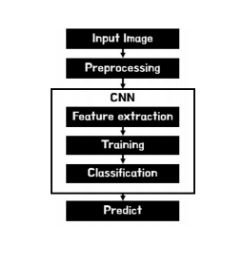
\includegraphics[height=18cm,width=15cm]{FLOWCHART.PNG}
\counterwithin{figure}{section}
%\counterwithout{figure}{chapter}
\caption{Proposed model architecture} 
\end{figure}


\subsection{Data Pre-Processing}
\paragraph{}
As the first step, Collecting sample images of fake and real fingerprint from the dataset provided by Liveness Detection Competition of the year 2015.It contains both training and tesing dataset. The training data set contains almost 50,000 real and fake fingerprints images.The quality of the fingerprint image are crucial for the recoginition process.
Initially we have to load both the training and testing datasets into our program.Then display the training images and its count.
\paragraph{}
The images are of different sizes. So we want to tranform the images into equal sizes.In Keras, image preprocessing task is performed by using ImageDataGenerator Class. Here perform resize, 
horizontalflip,shear,zooming operations.





\begin{figure}[H]
\centering
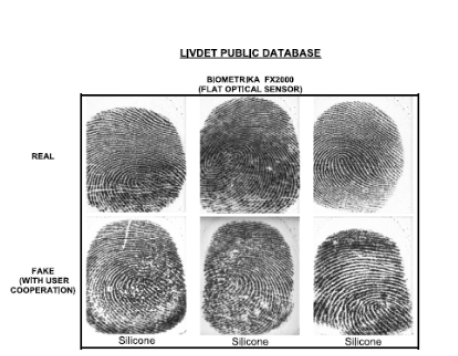
\includegraphics[height=14cm,width=15cm]{dataset.PNG}
\counterwithin{figure}{section}
%\counterwithout{figure}{chapter}
\caption{Examples of real and fake fingerprint images} 
\end{figure}







\subsection{CNN Modelling}

\paragraph{}
CNN Model consist of feature extraction, training and classification tasks.
Figure 3.3 illustrates the feed-forward pass of a single layer
convolutional network. The input sample is convoluted with
three random filters of size 5x5 (enlarged to make visualization
easier), generating 3 convoluted images, which are then subject
to non-linear function max(x; 0), followed by a max-pooling
operation, and subsampled by a factor of 2.


\begin{figure}[H]
\centering
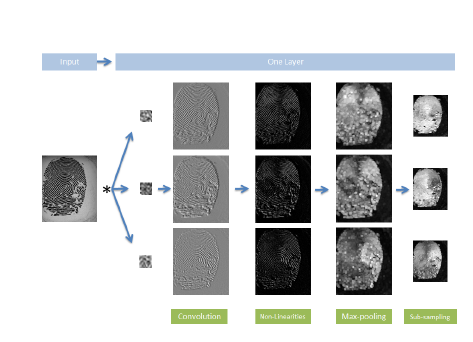
\includegraphics[height=18cm,width=15cm]{cnnfig.PNG}
\counterwithin{figure}{section}
%\counterwithout{figure}{chapter}
\caption{single layer convolutional network} 
\end{figure}



Here there are three main layers
\begin{itemize}
 
\item ReLU layer
\item Pooling Layer
\item Fully Connected Layer


\end{itemize}

\paragraph{}
Keras is used to model this network. Keras is a deep learning library in python. The core data structure of Keras is a model, a way to organize
layers. The simplest type of model is the Sequential model, a linear stack of layers. This model is initialised and the input image is pass throgh a convolution layer.ReLU is Rectified Linear Units. This layer applies the non-saturating activation function
f(x)=max(0,x). It increases the nonlinear properties of the decision function and of the overall network without affecting the receptive fields of the convolution layer.
\paragraph{}
Then it pass through a pooling layer.The pooling layer makes the CNN less sensitive to small changes
in the location of a feature. There are a number of ways to implement pooling, but the most effective is max pooling.
 Max pooling is also referred to as a downsampling layer.
Max pooling uses the maximum value from each of a cluster of
neurons at the prior layer. Max pooling reduces the size of feature map.To perform max pooling, imagine a window(size 2x2) sliding
across the feature map.
 As the window moves across the map, we take the largest value
in the window and discard the rest.
Then it pass through a fully connected network. Neurons in a fully connected layer have full connections to allactivations in the previous layer, as seen in regular NeuralNetworks
The fully-connected layer has 3 parts - an input layer, a hidden
layer, and an output layer. The input layer is the output of the preceding layer, which is just
an array of values.







\begin{figure}[H]
\centering
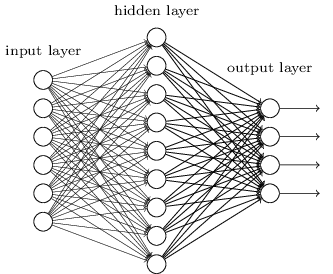
\includegraphics[height=15cm,width=12cm]{fullconn.png}
\counterwithin{figure}{section}
%\counterwithout{figure}{chapter}
\caption{Fully Connected Network} 
\end{figure}


\subsubsection{Training}
\paragraph{}
 Covolutional Neural Network can play a critical role in fingerprint liveness detection. An CNN can be configured and trained to handle such variations observed in the texture of the fingerprint. Extracted features of all the images in the data set are the input
of the neural network.
Here AdamOptimizer (Adaptive Moment Estimation) is used to get faster convergence.
AdamOptimizer is a type of Gradient Descent optimization algorithm. It is an optimization
algorithm that can used instead of the classical stochastic gradient descent procedure to update
network weights iterative based in training data.Here take 15 epochs for training and weight updation is performed.So loss can be calculated in each Epoch. Loss will be decreased while the training progressing. Based on the weight updation, a model is generated.



\subsubsection{Testing}
 Based on the generated model from training, testing is performed.
 To recognize the fingerprint take any image from the data set and
fed that image to the trained network.It gives the result by showing whether it matches to real or fake fingerprint and display the result.


\subsubsection{Prediction accuracy}
Compute the prediction accuracy based on the number of real and fake
images. Displaying the accuracy of the real and fake test dataset.

\begin{figure}[H]
\centering
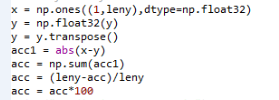
\includegraphics[height=10cm,width=10cm]{pred.PNG}
%\counterwithin{figure}{section}
%\counterwithout{figure}{chapter}
%caption{Training Dataset}
\end{figure}





\newpage
\section{EVALUATION}
\begin{itemize}
    \item Evaluation of the network using test dataset sample images.
\item Here we can find out the Accuracy of the Model.
\item In this, I have tested the model with 10 sample images.
\item Get the result whether the sample image is a fake or real fingerprint.
\item Compute the predicted accuracy.
 
    
    
\end{itemize}








\newpage
\section{CONCLUSIONS}
Convolutional Neural Networks were used to detect false vs real fingerprints. Pre-trained CNNs can yield state-of-the-art results on benchmark datasets without requiring architecture or hyper parameter selection. We also showed that these models have good accuracy on very small training sets (˜400 samples). Additionally, no task-specific hand-engineered technique was used as in classical computer vision approaches. Despite the differences between images acquired from different sensors, we show that training a single classifier using all datasets helps to improve accuracy and robustness. This suggests that the effort required to design a liveness detection system (such as hyper-parameters fine tuning) can be significantly reduced if different datasets (and acquiring devices) are combined during the training of a single classifier. Additionally, the pre-trained networks showed stronger generalization capabilities in cross-dataset experiments than CNN with random weights and the classic LBP pipeline.



\newpage
\cleardoublepage
\addcontentsline{toc}{section}{\textbf{References}}
\begin{thebibliography}{9}


\bibitem{d} V. Mura, L. Ghiani, G. L. Marcialis, F. Roli, D. A. Yambay, and
S. A. Schuckers,\emph{ “Livdet 2015 fingerprint liveness detection competition
2015.”}
\bibitem{d} J. Galbally, F. Alonso-Fernandez, J. Fierrez, and J. Ortega-Garcia,\emph{ “A
high performance fingerprint liveness detection method based on quality
related features,” }Future Generation Computer Systems, vol. 28, no. 1,
pp. 311–321, 2012.
\bibitem{d} Y. Chen, A. Jain, and S. Dass, \emph{“Fingerprint deformation for spoof
detection,” }in Biometric Symposium, 2005, p. 21.
\bibitem{d} B. Tan and S. Schuckers,\emph{ “Comparison of ridge-and intensity-based
perspiration liveness detection methods in fingerprint scanners,”} in
Defense and Security Symposium. International Society for Optics and
Photonics, 2006, pp. 62 020A–62 020A.
\bibitem{d} P. Coli, G. L. Marcialis, and F. Roli, \emph{“Fingerprint silicon replicas: static
and dynamic features for vitality detection using an optical capture
device,”} International Journal of Image and Graphics, vol. 8, no. 04,
pp. 495–512, 2008.
\bibitem{d} P. D. Lapsley, J. A. Lee, D. F. Pare Jr, and N. Hoffman, \emph{“Anti-fraud
biometric scanner that accurately detects blood flow,”} Apr. 7 1998, uS
Patent 5,737,439.
\bibitem{d}A. Antonelli, R. Cappelli, D. Maio, and D. Maltoni, \emph{“Fake finger detection
by skin distortion analysis,” }Information Forensics and Security,
IEEE Transactions on, vol. 1, no. 3, pp. 360–373, 2006.
\bibitem{d} Baldisserra, A. Franco, D. Maio, and D. Maltoni, \emph{“Fake fingerprint
detection by odor analysis,”} in Advances in Biometrics. Springer, 2005,
pp. 265–272.
\bibitem{d} A. K. Jain, Y. Chen, and M. Demirkus,\emph{ “Pores and ridges: Highresolution
fingerprint matching using level 3 features,”} Pattern Analysis
and Machine Intelligence, IEEE Transactions on, vol. 29, no. 1, pp.
15–27, 2007.

\bibitem{d}Purneet Kaur , Jaspreet Kaur {"Fingerprint Recognition Using Genetic Algorithm and Neural Network"} 
\bibitem{d}Aliyu Tukur {"Fingerprint Recognition and Matching" }

\bibitem{d}  Adrian Lim Hooi Jinl, Ai Chekima, Jamal Ahmad Dargham, and Liau Chung Fan {"Fingerprint identification and recognition using backpropagation neural network"}
\bibitem{d}Han-Ul Jang, Hak-Yeol Choi, Dongkyu Kim, Jeongho Son,and Heung-Kyu Lee {"Fingerprint Spoof Detection Using Contrast
Enhancement and Convolutional
Neural Networks"}

\bibitem{d}Diego Gragnaniello, Giovanni Poggi, Carlo Sansone and Luisa Verdoliva{"Fingerprint Liveness Detection
based on Weber Local Image Descriptor"}


\bibitem Tarang Chugh, Kai Cao, and Anil K. Jain, {"Fingerprint Spoof Buster"}


\bibitem Ravi Subban and Dattatreya P. Mankame
{"A Study of Biometric Approach Using Fingerprint
Recognition"} 

\bibitem W. F. Leung, S. H. Leung, W. H. Lau and Andrew Luk  {"Fingerprint recognition using neural network"}
\bibitem
Hriday Goyal, Gaurav Verma, Chetan Arora, { "Fingerprint Detection and Authentication using feature extraction based on Minutiae" }

\bibitem  Qiaoqiao Li,Patrick P. K. Chan, {"Fingerprint liveness detection based on binarized statistical image feature with sampling from Gaussian distribution"}

\bibitem{site1}https://ieeexplore.ieee.org/document/7390065/(Accessed On 18/03/18)



\end{thebibliography}
\newpage
\section{SCREENSHOTS}

\begin{figure}[H]
\centering
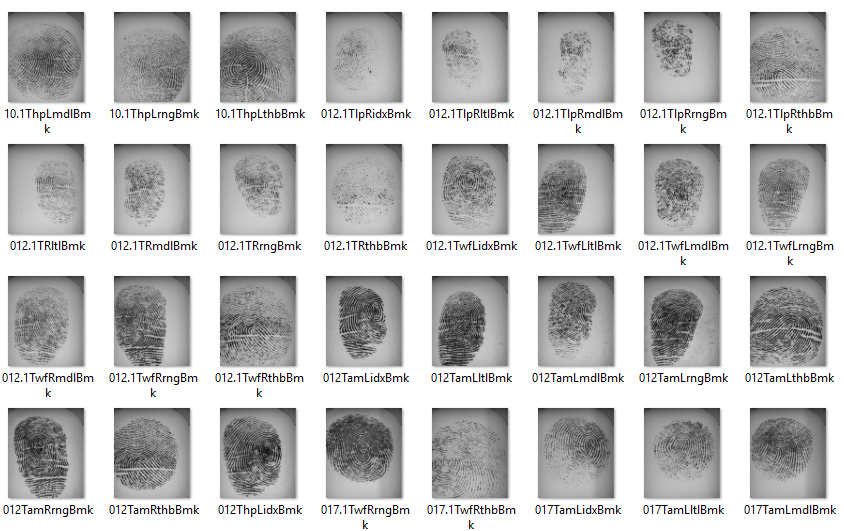
\includegraphics[height=10cm,width=15cm]{fingerinput.PNG}
\counterwithin{figure}{section}
%\counterwithout{figure}{chapter}
\caption{Training Dataset}
\end{figure}

\begin{figure}[H]
\centering
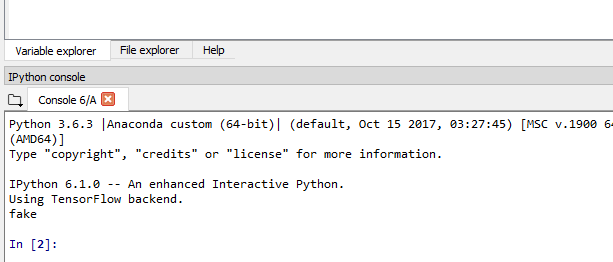
\includegraphics[height=10cm,width=15cm]{fingerout.png}
\counterwithin{figure}{section}
%\counterwithout{figure}{chapter}
\caption{Output }
\end{figure}



\begin{figure}[H]
\centering
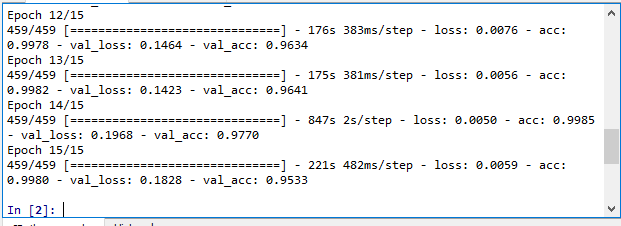
\includegraphics[height=10cm,width=15cm]{trainphto.PNG}
\counterwithin{figure}{section}
%\counterwithout{figure}{chapter}
\caption{Training Result }
\end{figure}



\begin{figure}[H]
\centering
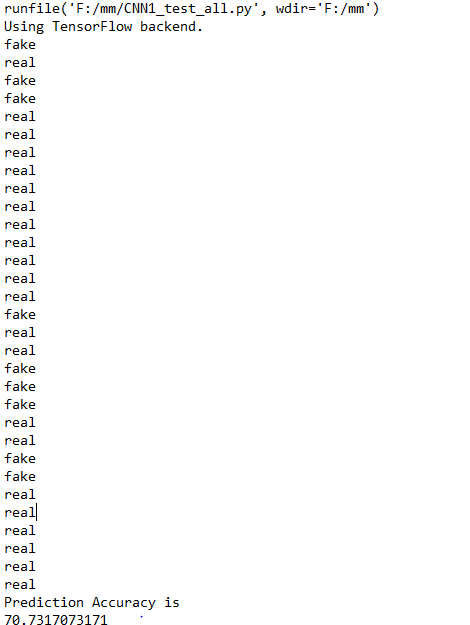
\includegraphics[height=10cm,width=15cm]{predct.PNG}
\counterwithin{figure}{section}
%\counterwithout{figure}{chapter}
\caption{Predicted Accuracy }
\end{figure}












\newpage
\section{APPENDIX}
\subsection{Code}

\textbf{Code for Training }
\begin{figure}[H]
\centering
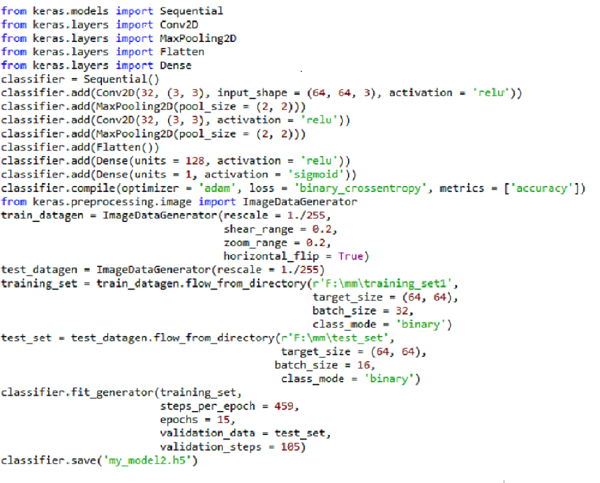
\includegraphics[height=20cm,width=15cm]{codecnn.PNG}
%\counterwithin{figure}{section}
%\counterwithout{figure}{chapter}
%caption{Training Dataset}
\end{figure}
\newpage
\textbf{Code for Testing }
\begin{figure}[H]
\centering
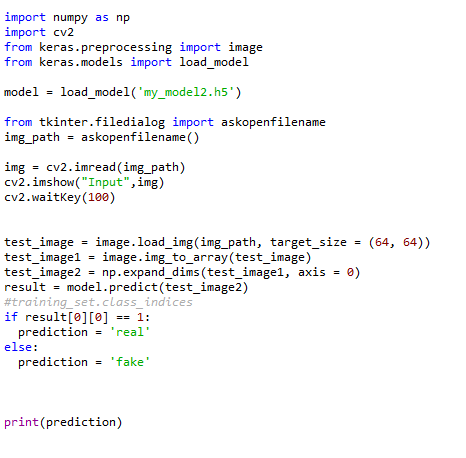
\includegraphics[height=20cm,width=15cm]{codetest.PNG}
%\counterwithin{figure}{section}
%\counterwithout{figure}{chapter}
%caption{Training Dataset}
\end{figure}
\newpage
\textbf{Prediction computing code}
\begin{figure}[H]
\centering
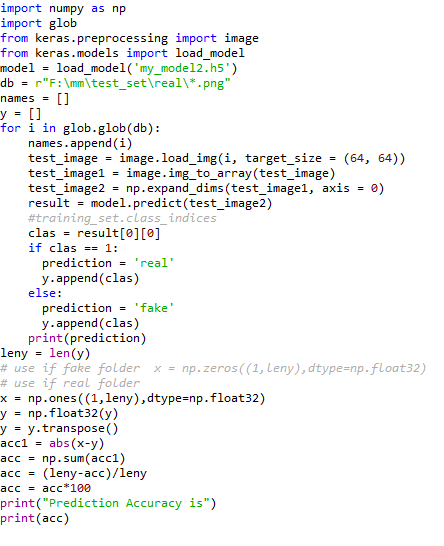
\includegraphics[height=20cm,width=15cm]{codetestall.PNG}
%\counterwithin{figure}{section}
%\counterwithout{figure}{chapter}
%caption{Training Dataset}
\end{figure}















\end{document}